\begin{minipage}{0.75\linewidth}
\begin{figure}[h]
    \centering
    \begin{adjustbox}{max width=1.0\linewidth, keepaspectratio}
        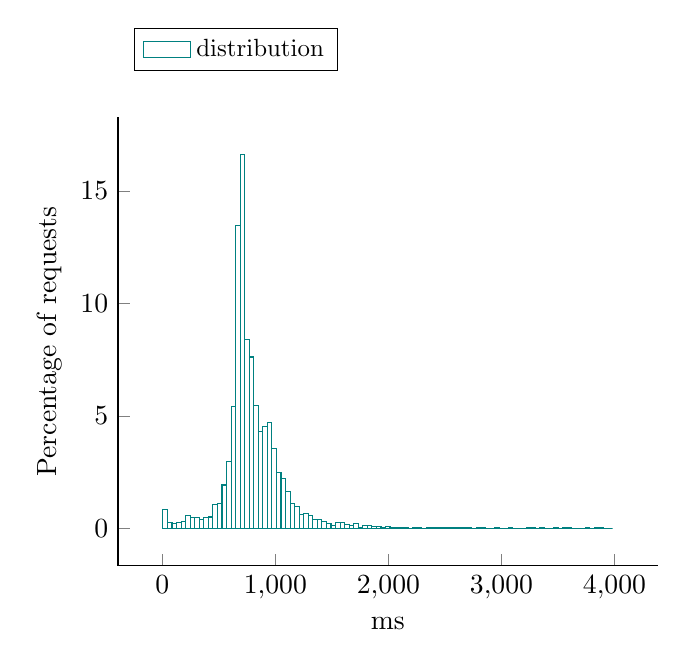
\begin{tikzpicture}
            \begin{axis}[ylabel = Percentage of requests, 
xlabel = ms, 
legend style = {nodes={scale=0.9, transform shape}, at={(0.03,1.2)}, anchor=north west, draw=black, fill=white, align=left, legend columns=3},
area style, mark size = 0pt,
 cycle list name = exotic,
  axis lines* = left]
		\addplot +[ybar interval] coordinates {
			 (5, 0.827485)
			 (45.19, 0.240913)
			 (85.38, 0.230439)
			 (125.57, 0.261862)
			 (165.76, 0.30376)
			 (205.95, 0.586572)
			 (246.14, 0.460878)
			 (286.33, 0.471352)
			 (326.52, 0.408505)
			 (366.71, 0.481827)
			 (406.9, 0.502776)
			 (447.09, 1.05792)
			 (487.28, 1.1103)
			 (527.47, 1.92731)
			 (567.66, 2.95381)
			 (607.85, 5.42579)
			 (648.04, 13.4597)
			 (688.23, 16.6125)
			 (728.42, 8.40054)
			 (768.61, 7.61496)
			 (808.8, 5.44674)
			 (848.99, 4.30502)
			 (889.18, 4.51451)
			 (929.37, 4.71352)
			 (969.56, 3.54038)
			 (1009.75, 2.46151)
			 (1049.94, 2.22059)
			 (1090.13, 1.65497)
			 (1130.32, 1.09982)
			 (1170.51, 0.953179)
			 (1210.7, 0.62847)
			 (1250.89, 0.638944)
			 (1291.08, 0.565623)
			 (1331.27, 0.408505)
			 (1371.46, 0.387556)
			 (1411.65, 0.293286)
			 (1451.84, 0.219964)
			 (1492.03, 0.115219)
			 (1532.22, 0.272337)
			 (1572.41, 0.240913)
			 (1612.6, 0.178066)
			 (1652.79, 0.125694)
			 (1692.98, 0.199015)
			 (1733.17, 0.0523725)
			 (1773.36, 0.115219)
			 (1813.55, 0.104745)
			 (1853.74, 0.083796)
			 (1893.93, 0.083796)
			 (1934.12, 0.020949)
			 (1974.31, 0.062847)
			 (2014.5, 0.0314235)
			 (2054.69, 0.0314235)
			 (2094.88, 0.041898)
			 (2135.07, 0.020949)
			 (2175.26, 0.0104745)
			 (2215.45, 0.041898)
			 (2255.64, 0.0314235)
			 (2295.83, 0)
			 (2336.02, 0.020949)
			 (2376.21, 0.0314235)
			 (2416.4, 0.041898)
			 (2456.59, 0.0314235)
			 (2496.78, 0.0523725)
			 (2536.97, 0.0523725)
			 (2577.16, 0.020949)
			 (2617.35, 0.020949)
			 (2657.54, 0.020949)
			 (2697.73, 0.0314235)
			 (2737.92, 0)
			 (2778.11, 0.020949)
			 (2818.3, 0.020949)
			 (2858.49, 0.0104745)
			 (2898.68, 0)
			 (2938.87, 0.020949)
			 (2979.06, 0.0104745)
			 (3019.25, 0.0104745)
			 (3059.44, 0.020949)
			 (3099.63, 0.0104745)
			 (3139.82, 0)
			 (3180.01, 0.0104745)
			 (3220.2, 0.0314235)
			 (3260.39, 0.020949)
			 (3300.58, 0.0104745)
			 (3340.77, 0.020949)
			 (3380.96, 0)
			 (3421.15, 0)
			 (3461.34, 0.020949)
			 (3501.53, 0.0104745)
			 (3541.72, 0.0314235)
			 (3581.91, 0.0314235)
			 (3622.1, 0)
			 (3662.29, 0)
			 (3702.48, 0)
			 (3742.67, 0.0314235)
			 (3782.86, 0.0104745)
			 (3823.05, 0.0314235)
			 (3863.24, 0.020949)
			 (3903.43, 0)
			 (3943.62, 0)
			 (3983.81, 0)
		};
\addlegendentry{distribution};
           \end{axis}
      \end{tikzpicture}
  \end{adjustbox}
  \caption{Response time distribution - req = ReadUser-2}
\end{figure}
\end{minipage}\hfill\begin{minipage}{0.18\linewidth}
\begin{table}[h]
\begin{tabular}{|cc|}
\hline
\textbf{} & \textbf{ms}\\ \hline
 \Xhline{0.005\arrayrulewidth}
min & 5\\
 \Xhline{0.005\arrayrulewidth}
max & 4024\\
 \Xhline{0.005\arrayrulewidth}
mean & 805\\
 \Xhline{0.005\arrayrulewidth}
std & 318\\
\hline
\hline
 \Xhline{0.005\arrayrulewidth}
25th & 671\\
 \Xhline{0.005\arrayrulewidth}
50th & 739\\
 \Xhline{0.005\arrayrulewidth}
75th & 905\\
 \Xhline{0.005\arrayrulewidth}
80th & 949\\
 \Xhline{0.005\arrayrulewidth}
85th & 996\\
 \Xhline{0.005\arrayrulewidth}
90th & 1079\\
 \Xhline{0.005\arrayrulewidth}
95th & 1258\\
 \Xhline{0.005\arrayrulewidth}
99th & 1986\\
\hline
\end{tabular}
\caption{Response time}
\end{table}
\end{minipage}\hfill